\documentclass{article}

\usepackage[T2A]{fontenc}
\usepackage[utf8]{inputenc}
% \usepackage[russian]{babel}
\usepackage{amsmath}
\usepackage{amssymb}
\usepackage{amsthm}
\usepackage{mathrsfs}

\usepackage{dan2e}

\usepackage{hyperref}       % hyperlinks
\usepackage{url}            % simple URL typesetting
\usepackage{booktabs}       % professional-quality tables
\usepackage{amsfonts}       % blackboard math symbols
\usepackage{nicefrac}       % compact symbols for 1/2, etc.
\usepackage{microtype}      % microtypography
\usepackage{lipsum}		% Can be removed after putting your text content
\usepackage{graphicx}
% \usepackage{natbib}
% \usepackage{doi}
\usepackage{mathtools}
\usepackage{xspace}	
\usepackage{amsthm}
\usepackage{setspace}
\usepackage{comment}
\usepackage{amsmath,amssymb}
\usepackage{algorithm}
\usepackage{algpseudocode}

\theoremstyle{definition}
\newtheorem{defi}{Определение}
\theoremstyle{plain}
% \newtheorem{remark}{Замечание}
% \newtheorem{theorem}{Теорема}

\newtheorem{theorem}{Theorem}
\newtheorem{corollary}{Corollary}[theorem]
\newtheorem{lemma}[theorem]{Lemma}

% my addition


\usepackage[english]{babel}
\usepackage[backend=biber,style=ieee,autocite=inline]{biblatex}
\bibliography{refs.bib}
\DefineBibliographyStrings{english}{%
  bibliography = {References},}
\DeclareFieldFormat{doi}{%
  doi\addcolon\space
  \ifhyperref
    {\lowercase{\href{https://doi.org/#1}{\nolinkurl{#1}}}}
    {\lowercase{\nolinkurl{#1}}}
}

\usepackage{graphicx}
\usepackage[symbol]{footmisc}
\renewcommand{\thefootnote}{\fnsymbol{footnote}}
\usepackage{float}
\usepackage{mathtools}
\usepackage{amssymb, amsmath, latexsym}
\usepackage{nicefrac}
\usepackage{hhline}
\usepackage{makecell}
\usepackage{caption}
\usepackage{multirow}
\renewcommand\theadalign{bc}
\renewcommand\theadfont{\bfseries}
\renewcommand\theadgape{\Gape[2pt]}
\renewcommand\cellgape{\Gape[2pt]}

\usepackage{colortbl}
\definecolor{bgcolor}{rgb}{0.8,1,1}
\definecolor{bgcolor2}{rgb}{0.8,1,0.8}
\usepackage{threeparttable}
\newcommand{\myred}[1]{{\color{red}#1}}
\newcommand{\myblue}[1]{{\color{blue}#1}}
% \usepackage[nocompress]{cite}
\usepackage{pifont}% http://ctan.org/pkg/pifont
\newcommand{\cmark}{\ding{51}}%
\newcommand{\xmark}{\ding{55}}%
\usepackage[colorinlistoftodos,bordercolor=orange,backgroundcolor=orange!20,linecolor=orange,textsize=scriptsize]{todonotes}
\usepackage{algorithm}\usepackage{algpseudocode}
\newcommand{\argmin}{\mathop{\arg\!\min}}
\newcommand{\argmax}{\mathop{\arg\!\max}}
\allowdisplaybreaks
\graphicspath{ {images/} }
% Used for displaying a sample figure. If possible, figure files should
% be included in EPS format.
%
% If you use the hyperref package, please uncomment the following line
% to display URLs in blue roman font according to Springer's eBook style:
% \renewcommand\UrlFont{\color{blue}\rmfamily}


% my addition end


\begin{document}

% TITLE START

\Volume{--}
\Year{2023}
\Pages{--}

\udk{--}

\title{Optimal data splitting in distributed optimization for machine learning}

\author{Medyakov Daniil\Addressmark[1],
Molodtsov Gleb\Addressmark[1],
Aleksandr Beznosikov\Addressmark[1],
Alexander Gasnikov\Addressmark[1]}

\Addresstext[1]{Moscow Institute of Physics and Technology, Dolgoprudny, Russia}

\Emailtext[1]{beznosikov.an@phystech.edu}

\markboth{D. Medyakov, G. Molodtsov, A. Beznosikov, A. Gasnikov}{Optimal data splitting in distributed optimization for machine learning}


% \presentedby{Представлено академиком Б.\,С.~Кашиным}

% \dateA{01.04.2022}
% \dateB{31.04.2022}
% \dateC{27.05.2022}


% \alttitle{Generalization of Landau and Becker--Pommerenke inequalities}

% \altauthor{O.\,S.~Kudryavtseva\Addressmark[a,b]\Emailmark[1], A.\,P.~Solodov\Addressmark[a]\Emailmark[2]}

% \altAddresstext[a]{Lomonosov Moscow State University, Moscow Center for Fundamental and Applied Mathematics, \\ Moscow, Russian Federation}

% \altAddresstext[b]{Volgograd State Technical University, Volgograd, Russian Federation}

% \altpresentedby{Presented by Academician of the RAS B.\,S.~Kashin}



\maketitle

% \doi{10.31857/S2686954322040117}

% ABSTRACT STARTS

\begin{abstract}
The distributed optimization problem has become increasingly relevant recently. It has a lot of advantages such as processing a large amount of data in less time compared to non-distributed methods. However, most distributed approaches suffer from a significant bottleneck -- the cost of communications. Therefore, a large amount of research has recently been directed at reducing these costs. One such approach uses local data similarity. In particular, an optimal method for distributed problems under the Hessian similarity condition has been proposed very recently. But this result, as well as results from other works solve the communication bottleneck by focusing only on the fact that communication is significantly more expensive than local computing and does not take into account the various capacities of network devices and the different relationship between communication time and server capacity. We consider this problem an the objective of this study is to achieve an optimal ratio of distributed data between the server and local machines for any communication costs and local computations. The running times of the network are compared between uniform and optimal distributions. The superior theoretical performance of our solutions is experimentally validated.
\end{abstract}


\section{Introduction}

\section*{1.1. Distributed optimization}

We consider optimization problems of the following form:
\begin{equation}
    \label{eq:1}
    \underset{x\in \mathbb{R}^d}{\min} ~ f(x) = \frac{1}{n} \sum \limits_{i = 1}^{n} f _i(x),
\end{equation}
$x\in\mathbb{R}^d$ collects the parameters of a statistical model to be trained, $n$ is the number of devices/nodes, and $f_i$ is the emperical risk of devices $i$, i.e., $f_i(x) = \frac{1}{b_i}\sum_{j = 1}^{b_i} l(x, z_i^j)$, where $z_i^1, \ldots ,z_i^{b_i}$ is set of $b_i$ samples owned by $i$-th device and $l(x, z_i^j)$ measures mismatch between the parameter $x$ and the sample $z_i^j$. This is a direct formulation of a distributed optimization problem. Nowadays, there are some reasons to consider this.

To achieve the best results in modern machine learning and minimization tasks, researchers and practitioners face various challenges. Training modern machine learning models remains an extremely challenging task, also because models are trained on increasingly large datasets. Having more data in the dataset increases the robustness and generalizability of the trained model. In this case, the data is typically processed using a network of devices, i.e., collected in a distributed manner and stored in edge nodes of the network, such as in classical clustering \cite{verbraeken2020survey} and federated  \cite{konevcny2016federated, li2020federated, kairouz2021advances} learning.

Several solution methods have been proposed to solve \eqref{eq:1}. The prototype approach involves interleaving edge devices calculations (nodes $i = 2, \ldots, n$) with communications to and from the server ($i = 1$), which maintains and updates the authoritative copy of the optimization variables, eventually producing the final solution estimate. In distributed learning of complex models, the communication overhead between devices in the network often becomes a bottleneck. Such a problem makes it necessary to develop more efficient distributed learning methods, some of which have been described in \cite{konevcny2016federated, ghosh2020communication, smith2018cocoa, gorbunov2021marina}.

\section*{1.2. Distributed optimization under similarity}

It is trendy today in machine learning to use momentum-based methods. One of the methods for solving a distributed optimization problem is the application of Nesterov acceleration \cite{nesterov2018lectures}, which is an optimal method for smooth non-distributed optimization problems. This method can be applicable to distributed networks as follows. At each iteration we will calculate the gradient locally and send the results to the server. The server will average the obtained gradients and make a method step. Then the number of communications will be equal to the number of iterations. In this case, we obtain optimal estimates for local computations -- $\sqrt{\kappa}, \kappa = \nicefrac{L}{\mu}$, where $L$ and $\mu$ are constants of smoothness and strong-convexity of target function $f$. In case $\kappa$ is small, this approach is acceptable. However, for ill-conditioned functions with a large $\kappa$, the polynomial dependence on $\kappa$ may be unsatisfactory, due to the high cost of communications. This is often the case for many empirical risk minimization (ERM) problems where the optimal regularization parameter for test predictive performance is very small.

To further improve communication complexity, we can exploit the additional structure typically found in ERM problems, known as function similarity \cite{arjevani2015communication, shamir2014communication, matsushima2014distributed}. One can define it as the difference of function gradients, i.e., $||\nabla f_i (x) - \nabla f_j (x)|| < \delta ~~  \forall x$. But this approach is not "natural", since if the problem is not bounded, such a $\delta$ cannot exist. Consider for example a quadratic problem: $\nexists~ \delta: \|(A_i - A_j)x\| < \delta~$  if $~ x\rightarrow \infty$. Therefore, we will consider a different approach: Hessian similarity. Specifically, for all $x$ in a suitable domain of interest and all $i \neq j; ~ i,j \in \{1,\ldots,n\}$, the difference between the Hessian matrices of local losses, denoted by $\|\nabla ^2 f_i(x) - \nabla ^2 f_j(x)\|$, is bounded by $\delta$, where $\delta > 0$ measures the degree of similarity. Under this assumption, we can estimate $\delta \sim \mathcal O(\nicefrac{1}{\sqrt{N}})$, where $N$ is the sample size per device \cite{arjevani2015communication}. This approach was used for the first time in \cite{shamir2014communication}.  After that, lower estimates were proved for this problem in \cite{arjevani2015communication}, where communication costs are proportional to $\sqrt{\nicefrac{\delta}{\mu}}$. Then for a long time researchers tried to find methods that would reach these estimates. Algorithms such as \cite{tian2022acceleration, sun2022distributed, reddi2016aide, hendrikx2020statistically, beznosikov2021distributed} have been obtained. In 2022, it was possible to obtain the optimal method which is described in \cite{kovalev2022optimal}. 

\section*{1.3. Various communication costs and local computations} \label{eq:1.3}

In these works, the assumption was made that communications cost significantly more than local computation. Moreover, in general, works on distributed optimization, not only in Hessian similarity, have made this assumption. We look at this question from a different angle. We will move away from fixed big communications and make 2 \textbf{assumptions}:
\begin{itemize}
    \item [1.] The devices in the network have different capacities, i.e., they perform local computations of the same amount of data for different times.
    \item [2.] The ratio of communication costs to local computation time is a variable value that can be either $\ll 1$, $\gg1$, or even $\sim 1$.
\end{itemize}
 Under such assumptions, we need a new approach to the distributed optimization problem based on the already obtained optimal algorithms.

Based on the above, in this paper we reply the question: 
\begin{center}
    \textit{ Can we find such a distribution of data among the devices in the network to reduce the actual running time of the optimal algorithm} \cite{kovalev2022optimal}\textit{~for any communication costs and local computations?}
\end{center}

In practice, networks can run for long periods of time and as a consequence, noise can occur. In other words, communication costs and device capacities are not constant values. In that way, we will make one more \textbf{assumption}:
\begin{itemize}
    \item [3.] We put communication costs and device capacities as random variables, start the network operation for a long time and measure their expectation and variance. Due to the fact that the distribution of data to devices depends on the constant communication time and device power, in reality, the optimal distribution will be different on account of noise. Therefore, this assumption raises the question of measuring the program running time error under the optimal data distribution.
\end{itemize}

\section*{1.4. Contributions}

In general, our contribution is as follows:
\begin{itemize}
    \item \textbf{Generalization of the computation model.} We build a general model for computing time in networks under distributed optimization. The model is based on the optimal algorithm \cite{kovalev2022optimal} and takes into account the different capacity of edge devices, various communication costs.
    \item \textbf{Comprehensive analysis.} We pay special attention to the limiting cases and obtain results in them. The case where communications are too expensive is not of practical interest as the whole idea of distributed learning is lost, but the case of inexpensive communications (not so expensive that the communication takes longer than processing all data by just one device) is of great interest. 
    \item \textbf{Different techniques for obtaining a solution.} We obtain results in different cases, including for different estimates of $\delta$. We use different techniques: Cardano's formula, upper estimates in limiting cases, finding the zero of the function using the simplest numerical methods.
    \item \textbf{Decision error due to noise.} Under the third assumption, we present the theoretical error of the program running time under communication and local capacities noise.
    \item \textbf{Experiments.} We also conducted experiments confirming that with the obtained distribution it takes less time to solve the selected problem. Besides, we conduct appropriate experiments with noise in the network.
\end{itemize}

\section{Problem Statement}

Let's stay under just the first two assumptions for now. To achieve lower communication and local gradient complexity, we can refer to Algorithm \ref{alg:1} from \cite{kovalev2022optimal}. For this purpose, the function must be represented as a sum of a smooth convex function $f_1$ and a smooth potentially non-convex function $f - f_1$. Then the algorithm will be rewritten in the following more general form:

\begin{algorithm}
\caption{Accelerated Extragradient}\label{alg:1}
\begin{algorithmic}
\item [1:] \textbf{Input:} $x^0 = x_f^0\in\mathbb R^d$
\item [2:] \textbf{Parameters:} $\tau\in (0, 1), \eta, \theta, \alpha > 0, K\in \{1, 2, \ldots\}$
\item [3:] \textbf{for~}$k = 0, 1, 2, \ldots, K-1$\textbf{~do}
\item [4:]    $\quad\quad x_g^k = \tau x^k + (1 - \tau)x_f^k$
\item [5:]    $\quad\quad x_f^{k+1} \approx \arg\underset{x\in\mathbb R^d}{\min} [A_{\theta}^k (x) := \langle \nabla (f - f_1)(x_g^k), x - x_g^k \rangle + \frac{1}{2\theta}\|x - x_g^k\|^2 + f_1(x)]$ 
\item [6:] $\quad\quad x^{k+1} = x^k + \eta\alpha(x_f^{k+1} - x^k) - \eta\nabla f(x_f^{k+1})$
\item [7:] \textbf{end for}
\item [8:] \textbf{Output:} $x^K$
\end{algorithmic}
\end{algorithm}

We need to analyze the work of this algorithm, namely, find out how many operations this algorithm performs per iteration. In line 5, when solving for the $\arg\min$ subproblem, one local computation is performed on devices to compute $f_i(x_g^k)$, followed by one communication to transmit these results, and additional computations to find the solution $x_f^{k+1}$. Then in line 6 there is one local computation, and one communication. We obtain an expression for the total running time of the algorithm. \\Let us introduce the following notations: $\tau_i$ -- time of one local computation on the i-th device, $K$ -- number of iterations, $\tau_{comm}$ -- time of one communication, $k_{some}$ -- additional computation of the central node, $n$ -- number of nodes in the network. Taking this into account, the total running time of the algorithm can be written as:\\
\begin{equation}
    \label{eq:3}
    T_{sum} = 2\cdot\max(\tau_1, \tau_2, \ldots, \tau_n)\cdot K + 2\cdot K\cdot\tau_{comm} + \tau_1\cdot k_{some}.
\end{equation}

Our task is to minimize the time $T_{sum}$. In view of the statement \eqref{eq:1} and the form of functions $f_i$ let us represent the time $\tau_i$ as $\tau_i = \tau_i^{loc}\cdot b_i$, where $\tau_i^{loc}$ is capacity, i.e., the time spent by the $i$-th device to process a unit of information submitted to its input, and $b_i$ is the size of dataset submitted to the $i$-th device. $b_i$ must satisfy the following constraints: $\sum\limits_{i = 1}^{n} b_i = N$, where $N$ is the size of the whole dataset, $\delta = \frac{L}{\sqrt{b_i}}$ or $\delta = \frac{L}{b_i}$ \cite{hendrikx2020statistically}.
Finally, we obtain the following optimization problem:
\begin{equation}
    \label{eq:4}
    \underset{\sum\limits_{i = 1}^{n} b_i = N; \delta = \frac{L}{{b_1}^{\gamma}}}{\min}[ 2\cdot\max(\tau_1^{loc}\cdot b_1, \tau_2^{loc}\cdot b_2, \ldots, \tau_n^{loc}\cdot b_n)\cdot K + 2\cdot K\cdot\tau_{comm} + \tau_1\cdot k_{some}], ~ \gamma \in \{\frac{1}{2}, 1\}.
\end{equation}

\section{How to solve (\ref{eq:4})}

\section*{3.1. The primary problem of minimization}
In \cite{kovalev2022optimal} the estimates of $K$ and $k_{some}$ are found, namely: \\ $2\cdot K = \mathcal O(\max\{1, \sqrt{\frac{\delta}{\mu}}\}log(\frac{1}{\varepsilon})), k_{some} = \mathcal O(\max\{1, \sqrt{\frac{L}{\delta}}, \sqrt{\frac{\delta}{\mu}}, \sqrt{\frac{L}{\mu}}\}\log(\frac{1}{\varepsilon}))$. \\

Thus, \eqref{eq:4} is reduced to:

\begin{eqnarray}
    \begin{split}
    \label{eq:5}
        \underset{\sum\limits_{i = 1}^{n} b_i = N; \delta = \frac{L}{{b_1}^\gamma}}{\min}[(\max(\tau_1^{loc}\cdot b_1, \tau_2^{loc}\cdot b_2, \ldots, \tau_n^{loc}\cdot b_n) + \tau_{comm}) \cdot \mathcal O(\max\{1, \sqrt{\frac{\delta}{\mu}}\log(\frac{1}{\varepsilon})\})  ~+
        \\ + ~
        \tau_1^{loc}\cdot b_1\cdot\mathcal O(\max\{1,\sqrt{\frac{L}{\delta}}, \sqrt{\frac{\delta}{\mu}}, \sqrt{\frac{L}{\mu}}\}\log(\frac{1}{\varepsilon}))] ,  ~ \gamma \in \{\frac{1}{2}, 1\}. \hspace{2.4cm}
    \end{split}
\end{eqnarray}

\section*{3.2. Auxiliary problem}
Consider an auxiliary problem:
\begin{equation}
    \label{eq:6}
    \underset{\sum\limits_{i = 2}^{n} b_i = N}{\min} [\max(\tau_2^{loc}\cdot b_2, \tau_3^{loc}\cdot b_3, \ldots, \tau_n^{loc}\cdot b_n)].
\end{equation}


\begin{lemma}
    \label{l1}
    The solution of problem \eqref{eq:6} is $\overrightarrow{b} = (b_2, b_3, \ldots, b_n)^{T}$ satisfying $\tau_2^{loc}\cdot b_2 = \tau_3^{loc}\cdot b_3 = \ldots = \tau_n^{loc}\cdot b_n$.
    \begin{proof}
        
        Without loss of generality, let us assume fixed values for $\tau_2^{loc}\leq \tau_3^{loc}\leq \ldots \leq \tau_n^{loc}$. \\
        Then let us arbitrarily choose $b_2\geq b_3\geq \ldots \geq b_n$.
        \\
        This is indeed the case, otherwise we would have a situation where $\exists ~ i \neq j: ~ i, j\in \{2, \ldots, n\} : \max(\tau_i^{loc}\cdot b_i, \tau_j^{loc}\cdot b_j) > \max(\tau_i^{loc}\cdot b_j, \tau_j^{loc}\cdot b_i)$, and therefore the distribution would be suboptimal. 
        \\
        Our goal is to minimize the function $g(\overrightarrow{b}) = \max(\tau_2^{loc}\cdot b_2, \tau_3^{loc}\cdot b_3, \ldots, \tau_n^{loc}\cdot b_n)$. 
        \\
        Suppose that there exists a distribution such that $\exists i \in \{2, \ldots, n\}: g(\overrightarrow{b}^0) = \tau_i^{loc}\cdot b_i^0$ is the minimum, and $\forall j: j \geq 2, j \neq i \hookrightarrow \tau_i^{loc}\cdot b_i^0 > \tau_j^{loc}\cdot b_j^0$. 
        \\
        It follows that $b_i^0 > \frac{\tau_j^{loc}}{\tau_i^{loc}}b_j^0 > \frac{\tau_{j_1}^{loc}}{\tau_i^{loc}}b_{j_1}^0 > \ldots > \frac{\tau_{j_k}^{loc}}{\tau_i^{loc}}b_{j_k}^0$. 
        \\
        Then, considering $\sum\limits_{i = 2}^n b_i = N \hookrightarrow b_i^0 + \frac{\tau_j^{loc}}{\tau_i^{loc}}b_j^0 + \frac{\tau_{j_1}^{loc}}{\tau_i^{loc}}b_{j_1}^0 + \ldots + \frac{\tau_{j_k}^{loc}}{\tau_i^{loc}}b_{j_k}^0 > N$,
        we obtain 
        \\
        $b_i^0 > N(1 + \tau_i^{loc}\sum\limits_{\substack{j = 2 \\ j \neq i}}^n \frac{1}{\tau_j^{loc}})^{-1}$.
        
        Next, let us consider $b_i = N(1 + \tau_i^{loc}\sum\limits_{\substack{j = 2 \\ j \neq i}}^n \frac{1}{\tau_j^{loc}})^{-1}, \quad b_j = \frac {\tau_i^{loc}}{\tau_j^{loc}}\cdot b_i  ~~ \forall j \in \{2,\ldots,n\}$. 
        This distribution yields a minimum of $g(\overrightarrow{b}) = \tau_i^{loc}\cdot b_i = \tau_j^{loc}\cdot b_j ~~ \forall j \in \{2,\ldots,n\}$, and $g(\overrightarrow{b}) < g(\overrightarrow{b}^0)$. 
        This contradicts the assumption of minimality. 
        \\
        Thus, for the distribution that minimizes the function $g(\overrightarrow{b}) = \max(\tau_2^{loc}\cdot b_2, \tau_3^{loc}\cdot b_3, \ldots, \tau_n^{loc}\cdot b_n)$, it holds that $\tau_2^{loc}\cdot b_2 = \tau_3^{loc}\cdot b_3 = \ldots = \tau_n^{loc}\cdot b_n$.
    \end{proof}
\end{lemma}
Let us return to the problem \eqref{eq:5}. In addition to the minimum expression already studied in \eqref{eq:6}, there are additional terms in the problem \eqref{eq:5}.  $\delta$ in \eqref{eq:5} depends on the value of $b_1$, but do not depend on $b_i, i = \overline{2, n}$. From this and Lemma \ref{l1}, it follows that in the original problem \eqref{eq:5}, the data sharing between the 2nd, 3rd, and subsequent devices should be proportional. Thus, the problem \eqref{eq:5} is reduced to a new problem with additional constraints:


\begin{eqnarray}
    \begin{split}
    \label{eq:7}
        \min_{\substack{\sum\limits_{i = 1}^{n} b_i = N; \delta = \frac{L}{{b_1}^\gamma};  \\
        \tau_2^{loc}\cdot b_2 = \ldots = \tau_n^{loc}\cdot b_n }} 
        [(\max(\tau_1^{loc}\cdot b_1, \tau_2^{loc}\cdot b_2, \ldots , \tau_n^{loc}\cdot b_n) + \tau_{comm})\cdot \mathcal O(\max\{1, \sqrt{\frac{\delta}{\mu}}\log(\frac{1}{\varepsilon})\}) ~+
        \\ + ~
        \tau_1^{loc}\cdot b_1\cdot\mathcal O(\max\{1,\sqrt{\frac{L}{\delta}}, \sqrt{\frac{\delta}{\mu}}, \sqrt{\frac{L}{\mu}}\}\log(\frac{1}{\varepsilon}))] ,  ~ \gamma \in \{\frac{1}{2}, 1\}. \hspace{2.4cm}
    \end{split}
\end{eqnarray}

    

\section*{3.3. Define the final minimization problem}
It follows from Lemma \ref{l1} that $b_i\cdot \tau_i^{loc} = const ~ \forall i \in \overline{2, n}$.
Therefore, $$ N - b_1 = \sum\limits_{i = 2}^{n} b_i = \sum\limits_{i = 2}^{n} \frac{\tau_2^{loc}\cdot b_2}{\tau_i^{loc}} = \tau_2^{loc}\cdot b_2 \cdot \sum\limits_{i = 2}^{n} \frac{1}{\tau_i^{loc}} \Rightarrow
b_2 = \frac{N - b_1}{\tau_2 ^{loc}}(\sum\limits_{i = 2}^{n} \frac{1}{\tau_i^{loc}})^{-1}.$$
As mentioned above, we will consider the case of $\delta = \frac{L}{b_1}$ and case of $\delta = \frac{L}{\sqrt{b_1}}$.
\section*{3.3.1. Case of $\delta = \frac{L}{b_1}$}

There the following relations are fulfilled:
\begin{equation}
    \notag
    \gamma = 1, \mu \leq \delta \leq L \Rightarrow 
    \\
    \notag
    \begin{cases}
      2\cdot K =  \mathcal O(\sqrt{\frac{L}{\mu b_1}}\log(\frac{1}{\varepsilon}))\\
      k_{some} = \mathcal O(\sqrt{\frac{L}{\mu}}\log(\frac{1}{\varepsilon}))
    \end{cases}\,.
\end{equation}
Substituting this estimates into \eqref{eq:7}  the problem will take the following form:
\begin{equation}
    \notag
    \underset{\sum\limits_{i = 1}^{n} b_i = N}{\min}[(\max\{\tau_1^{loc}\cdot b_1, \tau_2^{loc}\cdot b_2\} + \tau_{comm}) \cdot \mathcal O(\sqrt{\frac{L}{\mu {b_1}}}\log(\frac{1}{\varepsilon})) + \tau_1^{loc}\cdot b_1 \cdot \mathcal O(\sqrt{\frac{L}{\mu}}\log(\frac{1}{\varepsilon}))].
\end{equation}

As a result, leaving the only variable $b_1$ in the function we pass to the final form of minimization problem:

\begin{eqnarray}
    \begin{split}
    \label{eq:fm1}
        \underset{0 < b_1 \leq N}{\min}[(\max\{\tau_1^{loc}\cdot b_1; ~(N-b_1) \cdot (\sum\limits_{i = 2}^{n} \frac{1}{\tau_i^{loc}} )^{-1}\} + \tau_{comm}) \cdot \mathcal O(\sqrt{\frac{L}{\mu b_1}}\log(\frac{1}{\varepsilon})) ~+
        \\ + ~
        \tau_1^{loc}\cdot b_1 \cdot \mathcal O(\sqrt{\frac{L}{\mu}}\log(\frac{1}{\varepsilon}))]. \hspace{3.7cm}
    \end{split}
\end{eqnarray}
Let us investigate the problem further. To do this, find the point at which the expressions under the maximum coincide. 
\begin{equation}
    \notag
    b_1^0 \cdot (\tau_1^{loc} + (\sum\limits_{i = 2}^{n} \frac{1}{\tau_i^{loc}})^{-1}) = N (\sum\limits_{i = 2}^{n} \frac{1}{\tau_i^{loc}})^{-1} \Rightarrow b_1^0 = \frac{N (\sum\limits_{i = 2}^{n} \frac{1}{\tau_i^{loc}})^{-1}}{\tau_1^{loc} + (\sum\limits_{i = 2}^{n} \frac{1}{\tau_i^{loc}})^{-1}}.
\end{equation}
Thus, we obtained two half-intervals, on each of which we can formulate a different minimization problem:
\begin{eqnarray}
\label{half-int}
    \begin{cases}
    (a) ~ ~ 0 < b_1 \leq b_1^0 \Rightarrow \max\{\tau_1^{loc}\cdot b_1; ~(N-b_1) \cdot (\sum\limits_{i = 2}^{n} \frac{1}{\tau_i^{loc}} )^{-1}\} = 
    (N-b_1) \cdot (\sum\limits_{i = 2}^{n} \frac{1}{\tau_i^{loc}})^{-1}
    \\
    (b) ~ ~ b_1^0 <  b_1 \leq N \Rightarrow \max\{\tau_1^{loc}\cdot b_1; ~(N-b_1) \cdot (\sum\limits_{i = 2}^{n} \frac{1}{\tau_i^{loc}} )^{-1}\} = \tau_1^{loc}\cdot b_1
    \end{cases}\,.
\end{eqnarray}
We construct functions of one variable $\mathcal{F}_1(b_1), \mathcal{F}_2(b_1)$ on the corresponding half-intervals that need to be minimized according to problem \eqref{eq:fm1}. Besides immediately find their derivatives for further analysis.\\
$(a): ~\mathcal{F}_1(b_1) = [N (\sum\limits_{i = 2}^{n} \frac{1}{\tau_i^{loc}})^{-1} + \tau_{comm}]\cdot 
c_1 \sqrt{\frac{L}{\mu}}log (\frac{1}{\varepsilon})  b_1^{-\frac{1}{2}} - 
c_1  \sqrt{\frac{L}{\mu}}log (\frac{1}{\varepsilon})(\sum\limits_{i =
2}^{n} \frac{1}{\tau_i^{loc}})^{-1} b_1^{\frac{1}{2}}  + \tau_1^{loc}\cdot c_2  \sqrt{\frac{L}{\mu}}log (\frac{1}{\varepsilon}) b_1 $\\
$(b): ~\mathcal{F}_2(b_1) = \tau_{comm}\cdot 
c_1 \sqrt{\frac{L}{\mu}}log (\frac{1}{\varepsilon})  b_1^{-\frac{1}{2}} + 
c_1  \sqrt{\frac{L}{\mu}}log (\frac{1}{\varepsilon})\tau_1^{loc} b_1^{\frac{1}{2}}  + \tau_1^{loc}\cdot c_2  \sqrt{\frac{L}{\mu}}log (\frac{1}{\varepsilon}) b_1 $\\

$(a): ~\mathcal{F'}_1(b_1) = -\frac{1}{2}c_1 b_1^{-\frac{3}{2}}  [N (\sum\limits_{i = 2}^{n} \frac{1}{\tau_i^{loc}})^{-1} + \tau_{comm}]\cdot 
\sqrt{\frac{L}{\mu}}log (\frac{1}{\varepsilon})  - 
\frac{1}{2} c_1 b_1^{-\frac{1}{2}}   \sqrt{\frac{L}{\mu}}log (\frac{1}{\varepsilon})(\sum\limits_{i = 2}^{n} \frac{1}{\tau_i^{loc}})^{-1} +
\tau_1^{loc}\cdot c_2  \sqrt{\frac{L}{\mu}}log (\frac{1}{\varepsilon})$ \\
$(b): ~\mathcal{F'}_2(b_1) = -\frac{1}{2}c_1 b_1^{-\frac{3}{2}} \tau_{comm}\cdot \sqrt{\frac{L}{\mu}}log (\frac{1}{\varepsilon}) + \frac{1}{2} c_1 b_1^{-\frac{1}{2}}  \sqrt{\frac{L}{\mu}}log (\frac{1}{\varepsilon})\tau_1^{loc}   + \tau_1^{loc}\cdot c_2  \sqrt{\frac{L}{\mu}}log (\frac{1}{\varepsilon})$\\


\section*{3.3.2. Case of $\delta = \frac{L}{\sqrt{b_1}}$}
We will proceed similarly to the previous point. First, let us present the necessary relations in this case.
\begin{equation}
    \notag
    \gamma = \frac{1}{2}, \mu \leq \delta \leq L \Rightarrow 
    \\
    \notag
    \begin{cases}
      2\cdot K = \mathcal O(\sqrt{\frac{L}{\mu \sqrt{b_1}}}\log(\frac{1}{\varepsilon}))\\
      k_{some} = \mathcal O(\sqrt{\frac{L}{\mu}}\log(\frac{1}{\varepsilon}))
    \end{cases}\,.
\end{equation}
Substituting these relations into \eqref{eq:7}, we obtain

\begin{equation}
    \notag
    \underset{\sum\limits_{i = 1}^{n} b_i = N}{\min}[(\max\{\tau_1^{loc}\cdot b_1, \tau_2^{loc}\cdot b_2\} + \tau_{comm}) \cdot \mathcal O(\sqrt{\frac{L}{\mu \sqrt{b_1}}}\log(\frac{1}{\varepsilon})) + \tau_1^{loc}\cdot b_1 \cdot \mathcal O(\sqrt{\frac{L}{\mu}}\log(\frac{1}{\varepsilon}))].
\end{equation}

Again, getting rid of all variables except $b_1$ we write the final minimization problem in this case

\begin{eqnarray}
    \begin{split}
    \label{eq:fm2}
        \underset{0 < b_1 \leq N}{\min}[(\max\{\tau_1^{loc}\cdot b_1; ~(N-b_1) \cdot (\sum\limits_{i = 2}^{n} \frac{1}{\tau_i^{loc}} )^{-1}\} + \tau_{comm}) \cdot \mathcal O(\sqrt{\frac{L}{\mu \sqrt{b_1}}}\log(\frac{1}{\varepsilon})) ~+
        \\ + ~
        \tau_1^{loc}\cdot b_1 \cdot \mathcal O(\sqrt{\frac{L}{\mu}}\log(\frac{1}{\varepsilon}))]. \hspace{3.7cm}
    \end{split}
\end{eqnarray}
Similarly, we select the point $b_1^0$, it turns out to be the same as in the previous paragraph. After we can obtained two half-intervals, on each of which we can formulate a different minimization problem:
\begin{eqnarray}
\label{half-int}
    \begin{cases}
    (a) ~ ~ 0 < b_1 \leq b_1^0 \Rightarrow \max\{\tau_1^{loc}\cdot b_1; ~(N-b_1) \cdot (\sum\limits_{i = 2}^{n} \frac{1}{\tau_i^{loc}} )^{-1}\} = 
    (N-b_1) \cdot (\sum\limits_{i = 2}^{n} \frac{1}{\tau_i^{loc}})^{-1}
    \\
    (b) ~ ~ b_1^0 <  b_1 \leq N \Rightarrow \max\{\tau_1^{loc}\cdot b_1; ~(N-b_1) \cdot (\sum\limits_{i = 2}^{n} \frac{1}{\tau_i^{loc}} )^{-1}\} = \tau_1^{loc}\cdot b_1
    \end{cases}\,.
\end{eqnarray}
We construct functions of one variable $\mathcal{F}_1(b_1), \mathcal{F}_2(b_1)$ on the corresponding half-intervals that need to be minimized according to problem \eqref{eq:fm2}. Besides immediately find their derivatives for further analysis.\\
$(a): ~\mathcal{F}_1(b_1) = [N (\sum\limits_{i = 2}^{n} \frac{1}{\tau_i^{loc}})^{-1} + \tau_{comm}]\cdot 
c_1 \sqrt{\frac{L}{\mu}}log (\frac{1}{\varepsilon})  b_1^{-\frac{1}{4}} - 
c_1  \sqrt{\frac{L}{\mu}}log (\frac{1}{\varepsilon})(\sum\limits_{i =
2}^{n} \frac{1}{\tau_i^{loc}})^{-1} b_1^{\frac{3}{4}}  + \tau_1^{loc}\cdot c_2  \sqrt{\frac{L}{\mu}}log (\frac{1}{\varepsilon}) b_1 $\\
$(b): ~\mathcal{F}_2(b_1) = \tau_{comm}\cdot 
c_1 \sqrt{\frac{L}{\mu}}log (\frac{1}{\varepsilon})  b_1^{-\frac{1}{4}} + 
c_1  \sqrt{\frac{L}{\mu}}log (\frac{1}{\varepsilon})\tau_1^{loc} b_1^{\frac{3}{4}}  + \tau_1^{loc}\cdot c_2  \sqrt{\frac{L}{\mu}}log (\frac{1}{\varepsilon}) b_1 $
\\
$(a): ~\mathcal{F'}_1(b_1) = -\frac{1}{4}c_1 b_1^{-\frac{5}{4}}  [N (\sum\limits_{i = 2}^{n} \frac{1}{\tau_i^{loc}})^{-1} + \tau_{comm}]\cdot 
\sqrt{\frac{L}{\mu}}log (\frac{1}{\varepsilon})  - 
\frac{3}{4} c_1 b_1^{-\frac{1}{4}}   \sqrt{\frac{L}{\mu}}log (\frac{1}{\varepsilon})(\sum\limits_{i = 2}^{n} \frac{1}{\tau_i^{loc}})^{-1} +
\tau_1^{loc}\cdot c_2  \sqrt{\frac{L}{\mu}}log (\frac{1}{\varepsilon})$ \\
$(b): ~\mathcal{F'}_2(b_1) = -\frac{1}{4}c_1 b_1^{-\frac{5}{4}} \tau_{comm}\cdot \sqrt{\frac{L}{\mu}}log (\frac{1}{\varepsilon}) + \frac{3}{4} c_1 b_1^{-\frac{1}{4}}  \sqrt{\frac{L}{\mu}}log (\frac{1}{\varepsilon})\tau_1^{loc}   + \tau_1^{loc}\cdot c_2  \sqrt{\frac{L}{\mu}}log (\frac{1}{\varepsilon})$\\

\section*{3.4. Final solution in limiting cases}
\section*{3.4.1. Case of $~\delta = \frac{L}{b_1}$}\label{eq:3.4.1}
Our goal is to find the minimum of the already obtained functions $\mathcal{F}_1(b_1), \mathcal{F}_2(b_1)$. To do this, we will look for the zeros of $\mathcal{F'}_1(b_1), \mathcal{F'}_2(b_1)$. Here we obtain the cubic equation.
To solve it, we can use the Cardano formula.\\
Consider the equation $ax^{-\frac{1}{2}} + bx^{-\frac{3}{2}} + c = 0$,\\
where in cases $(a): ~ ~ 0 < b_1 \leq b_1^0 $ and $(b): ~ ~ b_1^0 <  b_1 \leq N$ we assume:
\begin{eqnarray}
\notag
    \begin{cases}
    (a): ~ ~ a = \frac{1}{2} c_1 \sqrt{\frac{L}{\mu}}log (\frac{1}{\varepsilon})(\sum\limits_{i = 2}^{n} \frac{1}{\tau_i^{loc}})^{-1}; ~
b = -\frac{1}{2} c_1 [N (\sum\limits_{i = 2}^{n} \frac{1}{\tau_i^{loc}})^{-1} + \tau_{comm}]\cdot 
\sqrt{\frac{L}{\mu}}log (\frac{1}{\varepsilon});\\
\quad\quad~~ c = \tau_1^{loc}\cdot c_2  \sqrt{\frac{L}{\mu}}log (\frac{1} {\varepsilon})
    \\
\notag
    (b): ~ ~ a = \frac{1}{2} c_1  \sqrt{\frac{L}{\mu}}log (\frac{1}{\varepsilon})\tau_1^{loc}; \quad 
b = -\frac{1}{2}c_1 \tau_{comm}\cdot \sqrt{\frac{L}{\mu}}log (\frac{1}{\varepsilon}); \quad 
c = \tau_1^{loc}\cdot c_2  \sqrt{\frac{L}{\mu}}log (\frac{1} {\varepsilon})
    \end{cases}\,.
\end{eqnarray}

Then on the condition that 

\begin{gather*}
    N \geq \frac{a^2}{3 c^2}+\frac{\sqrt[3]{2 a^6+3 \sqrt{3} \sqrt{4 a^3 b^3 c^6+27 b^4 c^8}+18 a^3 b c^2+27 b^2 c^4}}{3 \sqrt[3]{2} c^2}-  \\
    \frac{\sqrt[3]{2}\left(-a^4-6 a b c^2\right) } 
    {3 c^2 \sqrt[3]{2 a^6+3 \sqrt{3} \sqrt{4 a^3 b^3 c^6+27 b^4 c^8}+18 a^3 b c^2+27 b^2 c^4}}, \\
\end{gather*}

we get a solution: \\

\begin{gather*}
     x=\frac{a^2}{3 c^2}+\frac{\sqrt[3]{2 a^6+3 \sqrt{3} \sqrt{4 a^3 b^3 c^6+27 b^4 c^8}+18 a^3 b c^2+27 b^2 c^4}}{3 \sqrt[3]{2} c^2}- \\ \frac{\sqrt[3]{2}\left(-a^4-6 a b c^2\right)} 
    {3 c^2 \sqrt[3]{2 a^6+3 \sqrt{3} \sqrt{4 a^3 b^3 c^6+27 b^4 c^8}+18 a^3 b c^2+27 b^2 c^4}}.  \\
\end{gather*}

Hence the desired solution is trivially obtained. Since we have obtained one value of $b_1$ on each of the half-intervals, which is the minimum of the function on its, so by choosing the one on which the function is smaller, we obtain the desired $b_1$.

\section*{3.4.2. Case of $~\delta = \frac{L}{\sqrt{b_1}}$}\label{eq:3.4.2}
Proceed similarly to \ref{eq:3.4.1} does not work, since we cannot write out the solution of these equations in analytic form due to their powers.
Therefore, let us consider the following limiting cases:
\begin{enumerate}
    \item $\forall i\hookrightarrow \tau_{comm} \ll \tau_i^{loc};$
    \item $\forall i\hookrightarrow \tau_{comm} \gg \tau_i^{loc}, \forall i\neq j\hookrightarrow \tau_i^{loc} = \tau_j^{loc}.$
\end{enumerate}

Establish $\alpha = c_1\cdot\sqrt{\frac{L}{\mu}}\cdot \log(\frac{1}{\varepsilon}),\beta = c_2\cdot\sqrt{\frac{L}{\mu}}\cdot \log(\frac{1}{\varepsilon}) $.

\textbf{Consider case 1:}

\begin{itemize}
    \item [a)] $0 < b_1 \leq b_1^0\\$
    $~\mathcal{F}_1(b_1) = [N (\sum\limits_{i = 2}^{n} \frac{1}{\tau_i^{loc}})^{-1} + \tau_{comm}]\cdot 
    \alpha  b_1^{-\frac{1}{4}} - 
    \alpha(\sum\limits_{i =
    2}^{n} \frac{1}{\tau_i^{loc}})^{-1} b_1^{\frac{3}{4}}  + \tau_1^{loc}\cdot\beta b_1\\$
    Consider
    \begin{equation}
        \label{eq:9}
        \tau_1^{loc} \leq \tau_2^{loc} \leq\ldots \leq \tau_n^{loc}.
    \end{equation}
    Make the following estimate:

    \begin{eqnarray}
        \begin{split}
        \label{eq:10}
            (\sum\limits_{i = 2}^n \frac{1}{\tau_i^{loc}})^{-1} = \frac{1}{\frac{1}{\tau_1^{loc}} + \ldots + \frac{1}{\tau_n^{loc}}} = \hspace{2.7cm}
            \\ =~ 
            \frac{\tau_2^{loc}\cdot \ldots \cdot\tau_n^{loc}}{\tau_3^{loc}\cdot \ldots \cdot\tau_n^{loc} + \tau_2^{loc}\cdot \tau_4^{loc}\cdot\ldots \cdot\tau_n^{loc} + \ldots + \tau_2^{loc}\cdot \ldots \cdot\tau_{n-1}^{loc}} 
            \underset{\eqref{eq:9}}{\geq}
            \\ \underset{\eqref{eq:9}}{\geq}\frac{\tau_2^{loc}}{n - 1} \gg \tau_{comm}.\hspace{3.9cm}
        \end{split}
    \end{eqnarray}
   
    Given the estimate \eqref{eq:10}, the functions $\mathcal{F}_1(b_1), \mathcal{F'}_1(b_1)'$ are transformed as follows:
    \begin{eqnarray}
        \notag
        \begin{split}
            \mathcal{F}_1(b_1) = \alpha(\sum\limits_{i = 2}^n \frac{1}{\tau_i^{loc}})^{-1}\cdot b_1^{-\frac{1}{4}}(N - b_1) + \tau_1^{loc}\beta\cdot b_1
        \end{split}
    \end{eqnarray}
    \begin{equation}
    \notag
        \mathcal{F'}_1 (b_1) = \alpha(\sum\limits_{i = 2}^n \frac{1}{\tau_i^{loc}})^{-1}\cdot (-\frac{1}{4}b_1^{-\frac{5}{4}}N - \frac{3}{4}b_1^{-\frac{1}{4}}) + \tau_1^{loc}\beta.
    \end{equation}
    We get the equation in the same powers, and so again we cannot write out an analytic solution.

    \item[b)] $b_1^0\leq b_1\leq N\\$
    $\mathcal{F}_2(b_1) = \tau_{comm}\cdot 
    \alpha  b_1^{-\frac{1}{4}} + 
    \alpha\tau_1^{loc} b_1^{\frac{3}{4}}  + \tau_1^{loc}\cdot \beta b_1 =  \alpha\cdot b_1^{-\frac{1}{4}}(\tau_{comm} + \tau_1^{loc}b_1) + \beta\cdot\tau_1^{loc}\cdot b_1\\$
    Make the following estimate
    \begin{equation}
    \label{eq:11}
      \tau_1^{loc}b_1\underset{b_1\geq b_1^0, \eqref{eq:9}}{\geq} \frac{\tau_1^{loc}N\frac{\tau_2^{loc}}{n - 1}}{\tau_1^{loc} + \frac{\tau_n^{loc}}{n - 1}}\geq \frac{\tau_1^{loc}\tau_2^{loc}N}{(n - 1)(\tau_1^{loc} + \tau_n^{loc})}\geq \frac{\tau_1^{loc}\tau_2^{loc}N}{2(n - 1)\tau_n^{loc}} \gg
    \end{equation}
    \begin{equation}
         \notag
         \gg ~
       \tau_{comm}\frac{N}{2(n - 1)} \gg \tau_{comm}.
    \end{equation}
    Then taking into account \eqref{eq:11}:
    \begin{equation}
        \notag
        \mathcal F_2(b_1) = \alpha\cdot\tau_1^{loc}\cdot b_1^{\frac{3}{4}} + \beta \tau_1^{loc}\cdot b_1
    \end{equation}
    \begin{equation}
        \notag
        \mathcal{F'}_2(b_1) = \frac{3}{4}\alpha\cdot\tau_1^{loc\cdot} b_1^{-\frac{1}{4}} + \beta\cdot\tau_1^{loc} > 0.
    \end{equation}
    Since the derivative of the function is positive, the function is increasing, and therefore the minimum will be taken at $b_1 = b_1^{0} = \frac{N (\sum\limits_{i = 2}^{n} \frac{1}{\tau_i^{loc}})^{-1}}{\tau_1^{loc} + (\sum\limits_{i = 2}^{n} \frac{1}{\tau_i^{loc}})^{-1}}.$  
Thus, in the case of small $\tau_{comm}$ we obtained the following result:\\
$b_{1_{\min}} \leq b_1^0 = \frac{N (\sum\limits_{i = 2}^{n} \frac{1}{\tau_i^{loc}})^{-1}}{\tau_1^{loc} + (\sum\limits_{i = 2}^{n} \frac{1}{\tau_i^{loc}})^{-1}}$.
\end{itemize}

\textbf{Consider case 2:}
\begin{itemize}
\item []
Establish: $\tau := t_i^{loc}~ \forall i \in {1,\ldots, n} $. 
\begin{equation}
        \text{Then} ~ ~\mathcal{F} = (\max\{\tau b_1; (N-b_1) \frac{\tau}{n-1}\} + \tau_{comm}) \cdot \frac{\alpha}{\sqrt[4]{b_1}}+\tau \beta b_1. 
\end{equation}

Consider the case $\tau_{comm} = N^2 \tau$ . $N$ can be considered large, so $\tau_{comm} \gg N\tau$. Then:
\begin{equation}
    \notag
     \max \{\tau b_1; (N-b_1)\frac{\tau}{n-1}\} < \tau N \ll \tau_{comm}\Rightarrow \mathcal{F} \approx \frac{\alpha \tau_{comm}}{\sqrt[4]{b_1}} + \beta \tau b_1 
\end{equation}
\begin{equation}
    \notag
    \mathcal{F}' (b_1) = -\frac{\alpha \tau_{comm}}{4b_1\sqrt[4]{b_1}} + \beta \tau = 0 \Rightarrow b_{1_{\min}}^\frac{5}{4} = \frac{\tau _{comm}\alpha}{4\beta\tau}\Rightarrow b_{1_{\min}} = (\frac{\tau _{comm}\alpha}{4\beta\tau})^{\frac{4}{5}}.
\end{equation}
Assuming that the found value $b_1$ lies on the interval $(0, N) $, that is, at $0 < (\frac{\tau _{comm}\alpha}{4\beta\tau})^{\frac{4}{5}} < N$, it will be the point of minimum function $\mathcal{F}$. Then:
\begin{equation}
    \notag
    \mathcal{F}(b_{1_{\min}}) = (\alpha \tau_{comm})^\frac{4}{5} \cdot (4\beta\tau)^\frac{1}{5} + (\beta \tau)^\frac{1}{5}\cdot(\frac{\alpha \tau_{comm}}{4})^\frac{4}{5} = (\alpha \tau_{comm})^\frac{4}{5}\cdot (\beta\tau)^\frac{1}{5}(4^\frac{1}{5} + 4^{-\frac{4}{5}}).
\end{equation}
    
Otherwise, the minimum will be reached at the right boundary, since at zero we can say that the function is increasing.
    \\
Summarizing all of the above in this case, it is worth noting that for very large values of $N$ the second special case generalizes to the following condition:

\begin {equation} 
    \forall i  \hookrightarrow \tau_{comm} = \mathcal{O}( N^k \tau_i^{loc}), k >1 , \forall i\neq j\hookrightarrow \tau_i^{loc} = \tau_j^{loc}
\end {equation}
\begin {equation}          
\min ~ {\mathcal{F}}(b_1) = \begin{cases}
      (\alpha \tau_{comm})^\frac{4}{5}\cdot (\beta\tau)^\frac{1}{5}(4^\frac{1}{5} + 4^{-\frac{4}{5}}),  0 < (\frac{\tau _{comm}\alpha}{4\beta\tau})^{\frac{4}{5}} < N\\
      \frac{\alpha\tau _{comm}}{N} + \beta \tau N , (\frac{\tau _{comm}\alpha}{4\beta\tau})^{\frac{4}{5}} \geq N
    \end{cases}\,.
\end {equation}
\end{itemize}

\section*{3.5. Practical solution}\label{eq:3.5}
Since an analytical solution is not found for all cases, we give a general numerical solution to our problem. In order to determine the minimum of these functions on the respective half-intervals, we will examine points where the derivatives of $\mathcal{F'}_1(b_1)$ and $\mathcal{F'}_2(b_1)$ approach zero. It should be noted that, given the nature of these functions, their derivatives can only be zero once on the desired half-interval. Hence, by employing Newton's method \cite{polyak2007newton} for $\mathcal{F'}_1(b_1)$ and $\mathcal{F'}_2(b_1)$, we can locate its zeros. Subsequently, we need to compare the values of the corresponding function at these points with the value at the extreme point of the interval. One of these points will provide the minimum solution, thereby serving as the ultimate solution to the problem \eqref{eq:fm1} and \eqref{eq:fm2}.

\section{Noise in the networks}

Now we proceed to the third assumption from the \ref{eq:1.3}. As mentioned above, let $\tau_{comm}$ and $\tau_i^{loc}$ be random variables: $\exists ~\mathbb E [\tau_{comm}], \mathbb E [\tau_i^{loc}], \mathbb D [\tau_{comm}] < \infty, \mathbb D [\tau_i^{loc}] < \infty$. Here we consider case of $\delta = \frac{L}{\sqrt{b_1}}$. The analytical solution in this set up was obtained in the limiting cases for small and large communications, with respect to local computation time. Let us consider them separately. 

\section*{4.1. Case of big communication time}\label{s:4.1}

Allow us impose additional constraints on the random variables $\tau_{comm}$ and $\tau_i^{loc}$: $\forall \{\tau_{comm}^k\}_{k = 1}^m, \{\tau_{i}^{loc, ~k}\}_{k = 1}^m~\forall k, i \hookrightarrow \tau_{comm}^k \gg \tau_{i}^{loc, ~k}$. Consider the function of task running time \eqref{eq:fm2} at the point of minimum. Earlier in \ref{eq:3.4.2} it was obtained:
\begin{equation}
    \label{eq:17}
    \mathcal{F}(b_{1_{\min}}) = (\alpha\cdot\tau_{comm})^{\nicefrac{4}{5}}\cdot (\beta\cdot\tau_1^{loc})^{\nicefrac{1}{5}}\cdot(4^{\nicefrac{1}{5}} + 4^{-\nicefrac{4}{5}}).
\end{equation}

To obtain the result, we produce the following equality: $X, Y -$  independent random variables $\Rightarrow \mathbb D [XY] = \mathbb E [(XY - \mathbb E[XY])^2] = \mathbb E[(XY)^2] - 2\mathbb E^2 [XY] + \mathbb E^2[XY] = \mathbb E[X^2]\mathbb E[Y^2] - \mathbb E^2 [X]\mathbb E^2 [Y] = (\mathbb D [X] + \mathbb E^2 [X])\cdot(\mathbb D [Y] + \mathbb E^2 [Y]) - \mathbb E^2 [X]\mathbb E^2 [Y] = \mathbb D[X]\mathbb D[Y] + \mathbb D[X]\mathbb E^2 [Y]  + \mathbb D[Y]\mathbb E^2 [X]$. Applying this equality to \eqref{eq:17} we get the error we are looking for:
\begin{eqnarray}
    \begin{split}
    \label{eq:18}
        \mathbb D [\mathcal{F}(b_{1_{\min}})] = [\alpha^{\nicefrac{4}{5}}\cdot\beta^{\nicefrac{1}{5}}\cdot(4^{\nicefrac{1}{5}} + 4^{-\nicefrac{4}{5}})]\cdot\{\mathbb D [(\tau_{comm})^{\nicefrac{4}{5}}]\mathbb D [(\tau_1^{loc})^{\nicefrac{1}{5}}]~+
        \\ + ~ \vspace{3cm}
         \mathbb D [(\tau_{comm})^{\nicefrac{4}{5}}]\mathbb E^2 [(\tau_1^{loc})^{\nicefrac{1}{5}}] + \mathbb D [(\tau_1^{loc})^{\nicefrac{1}{5}}]\mathbb E^2 [(\tau_{comm})^{\nicefrac{4}{5}}]\}.  \hspace{1.5cm}
    \end{split}
\end{eqnarray}

\section*{4.2. Case of small communication time}

Here we will consider noise only on communications, i.e. we will put the time of communications as a random variable with mathematical expectation and finite variance, and the time of local computations for each device as a constant value. Similarly to the previous paragraph we impose additional constraints: $\forall \{\tau_{comm}^k\}_{k = 1}^m~\forall k, i \hookrightarrow \tau_{comm}^k \ll \tau_{i}^{loc}$. Consider the function of task running time \eqref{eq:fm2} at the point of minimum (here we'll take the point $b_1^0$):
\begin{eqnarray}
    \begin{split}
        \mathcal{F}(b_{1_{\min}}) = [(N - b_1^0)\cdot(\sum\limits_{i = 2}^n \frac{1}{\tau_i^{loc}})^{-1} + \tau_{comm}]\cdot\alpha\cdot\frac{1}{(b_1^0)^{\nicefrac{1}{4}}} + \tau_1^{loc}\cdot b_1^0\cdot\beta ~= 
        \\ =~
        \left[\frac{\tau_1^{loc}\cdot N\cdot (\sum\limits_{i = 2}^n \frac{1}{\tau_i^{loc}})^{-1}}{\tau_1^{loc} + (\sum\limits_{i = 2}^n \frac{1}{\tau_i^{loc}})^{-1}} + \tau_{comm}\right]\cdot\alpha\cdot\frac{(\tau_1^{loc} + (\sum\limits_{i = 2}^n \frac{1}{\tau_i^{loc}})^{-1})^{\nicefrac{1}{4}}}{(N\cdot (\sum\limits_{i = 2}^n \frac{1}{\tau_i^{loc}})^{-1})^{\nicefrac{1}{4}}} + \tau_1^{loc}\cdot b_1^0\cdot\beta.
    \end{split}
\end{eqnarray}

Then the error required will be as follows:
\begin{equation}
    \label{eq:20}
    \mathbb D [\mathcal{F}(b_{1_{\min}})] = \left[\alpha\cdot\frac{(\tau_1^{loc} + (\sum\limits_{i = 2}^n \frac{1}{\tau_i^{loc}})^{-1})^{\nicefrac{1}{4}}}{(N\cdot (\sum\limits_{i = 2}^n \frac{1}{\tau_i^{loc}})^{-1})^{\nicefrac{1}{4}}}\right]^2\cdot \mathbb D [\tau_{comm}].
\end{equation}


\section{Experiments}

\section*{5.1. Experiments with data distribution}
For experimental verification of the theoretical results we consider the ridge regression problem: 
\begin{equation}
    \label{ridge}
    \underset{\omega}{\min}[ \frac{1}{2N} \|X\omega - y\|_2^2 + \frac{\lambda}{2}\|\omega\|_2^2],
\end{equation}
where $\omega$ is the vector of weights of the model, $\{x_i, y_i\}_{i = 1}^N$ is the training dataset, and $\lambda > 0$ is the regularization parameter. We consider a network  with 21 workers simulated on a single-CPU machine. We use dataset from LIBSVM library \cite{chang2011libsvm}. Value $\tau_1^{loc} = 1$, values for other i $\tau_i^{loc}, i \neq 1$ were taken conditionally and generated uniformly from 3 to 7. $\tau_{comm}$ were chosen so that $\frac{\tau _{comm}}{\tau _1^{loc}} = 10^l, l = \overline{-6, 12}$

\begin{comment}
In the first stages $\arg\underset{x}{\min} [p(x_k^g) + <\nabla p(x_k^g), x - x_k^g> + \frac{1}{2\Theta}||x - x_k^g||^2 + q(x)]$ was searched explicitly (Line 5 of Algorithm 1). This was done by equating the gradient to zero. Applying to the problem \ref{ridge}: 
\begin{center}
$\nabla p(\omega_k^g) + \frac{1}{\Theta}(x - \omega_k^g) + \nabla q(x) = 0 \Rightarrow \lambda \omega_k^g + \frac{1}{\Theta}(Ix - \omega_k^g) + \frac{1}{N}X^T(Xx - y) = 0 \Rightarrow$

    
$ x = (I \frac{1}{\Theta} + \frac{1}{N}X^TX)^{-1}(\frac{1}{\Theta} \omega_k^g + \frac{1}{N}X^Ty - \lambda \omega_k^g) $
\end{center}

Then in Algorithm 1 on line 5: $x_f^{k+1} = x$
\end{comment}
 We implemented Algorithm \ref{alg:1} in Python 3.9.6 using the iterative OGM-G method from \cite{kim2021optimizing} to find the $\arg\min$ in \ref{alg:1}. That is what the original article \cite{kovalev2022optimal} recommends. After calculating the required number of iterations to achieve a certain accuracy we find the values of constants $c_1, c_2$, and, respectively, $\alpha, \beta$. With their help, we were able to distribute the data from the dataset to the devices according to the above formulas. 

Next, we ran the algorithm and measured the running time on the resulting distribution of data across devices and uniform distribution. The cases of large and small communications were considered. 

In the end, two cases were considered: 
\begin{enumerate}
    \item $\delta = \frac{L}{\sqrt{b_1}}$;
    \item $\delta = \frac{L}{b_1}$.
\end{enumerate}

For case 1, following setups were considered:
\begin{enumerate}
    \item small communications ($b_1 = b_1^0$) \hyperref[eq:3.4.2]{3.4.2};
    \item large communications \hyperref[eq:3.4.2]{3.4.2};
    \item search for optimal allocation using Newton's method \hyperref[eq:3.5]{3.5}.
\end{enumerate}

For case 2, following setups were considered:
\begin{enumerate}
    \item search for the optimal solution using the Cardano formula \hyperref[eq:3.4.1]{3.4.1};
    \item search for optimal allocation using Newton's method \hyperref[eq:3.5]{3.5}.
\end{enumerate}

For all cases, acceleration was found and plots were shown at \ref{ris:image}.

\begin{figure}[!ht]
    {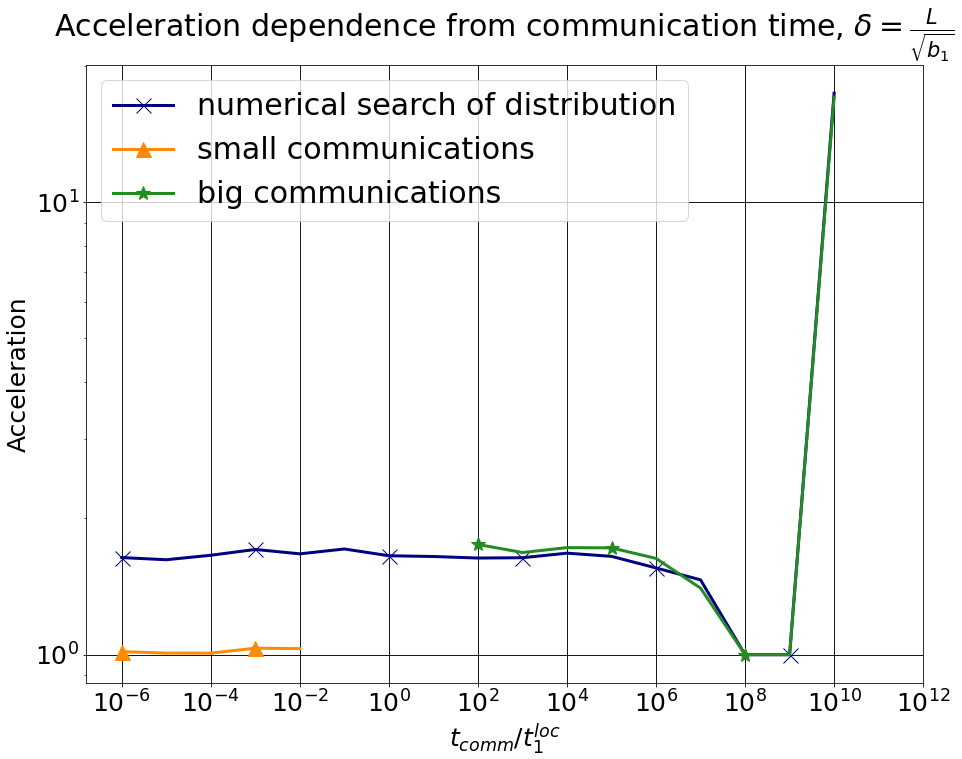
\includegraphics[scale = 0.25]{график11.png}}
    {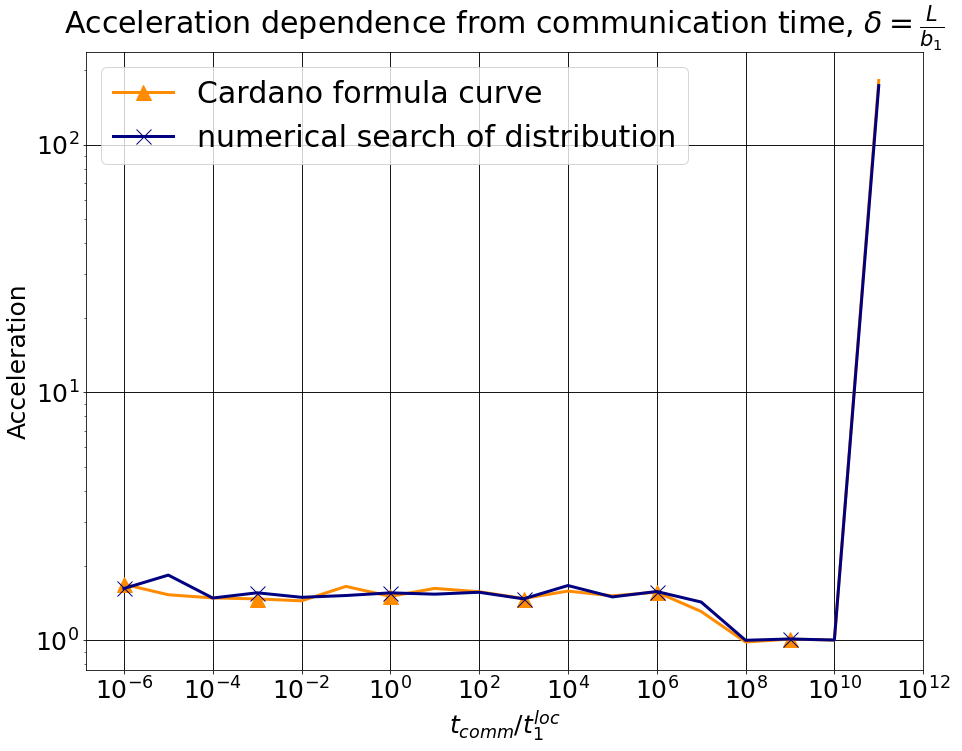
\includegraphics[scale = 0.25]{график22.png}}
    \caption{Experiments with data distribution}
    \label{ris:image}
\end{figure}


%\begin{figure}[h]
%\center{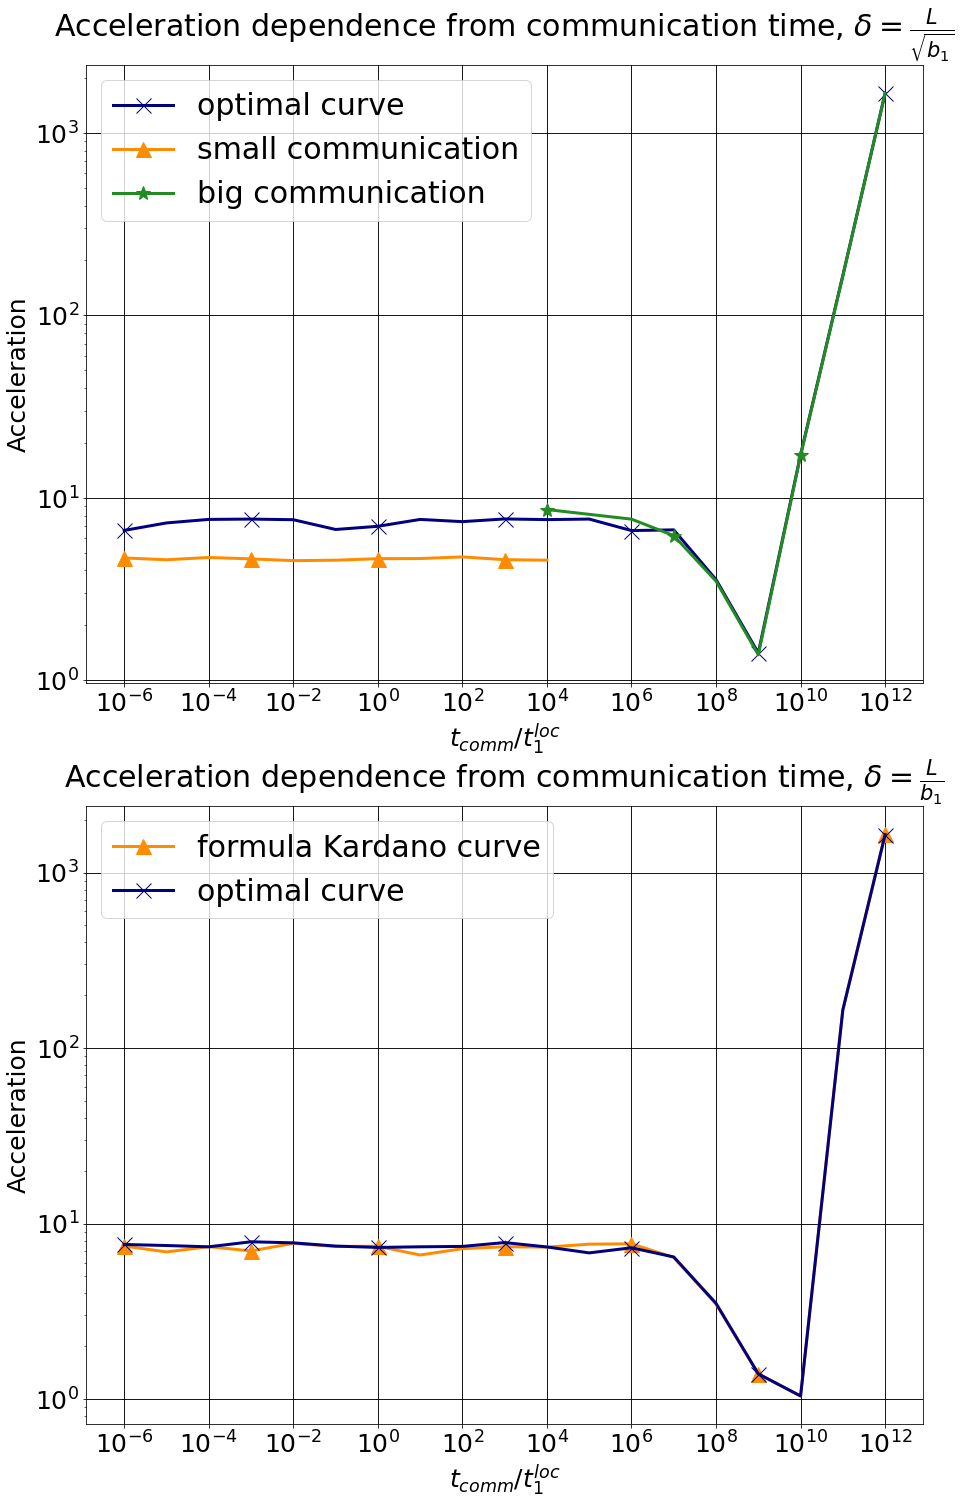
\includegraphics[width=0.8\linewidth]{final_graph.png}}
%\caption{Final results}
%\label{ris:image}
%\end{figure}

\section*{5.2. Analyze}
Let us analyze the obtained plots. The formula for the case of large communications and the Cardano formula practically coincided with the optimal solution search. The case of small communications showed worse results. This is explained by the fact that the formula was obtained in rough approximation. But if we take into account the constants $\alpha, \beta$, we can get a better result, which is shown below.



\begin{gather*}
    F=\left(\max \left\{\tau_1^{loc} \cdot b_1 ;\left(N-b_1\right) \cdot\left(\sum_{i=2}^n \frac{1}{\tau_i^{loc}}\right)^{-1}\right\}+\tau_{comm}\right) \cdot \frac{\alpha}{\sqrt[4]{b_1}}+\tau_1^{loc} b_1 \cdot \beta \\
    \text {It has already been evaluated that } b_1 \leq b_1^0 \Rightarrow F=\left(N-b_1\right)\cdot \left(\sum_{i=2}^n \frac{1}{\tau_i^{loc}}\right)^{-1} \cdot \frac{\alpha}{\sqrt[4]{b_1}}+\tau_1^{loc} b_1 \cdot \beta.
\end{gather*}


\begin{gather*}
    F=N\left(\sum_{i=2}^n \frac{1}{\tau_i^{loc}}\right)^{-1} \alpha b^{-\frac{1}{4}}-\left(\sum_{i=2}^n \frac{1}{\tau_i^{loc}}\right)^{-1} \alpha b_1^{\frac{3}{4}}+\tau_1^{l o c} \beta b_1. \\
    \text {Consider that} \quad \alpha \sim 10^6, \beta \sim 10^9 \Rightarrow \\ 
    F \cong 10^6 N \left(\sum_{i=2}^n \frac{1}{\tau_i^{loc}}\right)^{-1} \cdot b^{-\frac{1}{4}}-10^6 \left(\sum_{i=2}^n \frac{1}{\tau_i^{loc}}\right)^{-1} \cdot b_1^{\frac{3}{4}}+10^9 \tau_1^{loc} b_1, \\
    \frac{1}{4} \cdot 10^6 N \left(\sum_{i=2}^n \frac{1}{\tau_i^{loc}}\right)^{-1} \cdot b_1^{-\frac{5}{4}} \ \leq 10^5 \tau_1^{loc} \Rightarrow b_1 \leq \frac{4 \cdot 10^3 \tau_1^{loc}}{N\left(\sum_{i=2}^n\left(\tau_i^{loc}\right)^{-1}\right)^{-1}}.
\end{gather*}

\section*{5.3. Experiments with noise in the network}

We modified the simulation of Algorithm \ref{alg:1} by adding communication  and device power noise. We generated the noise from a uniform distribution and its value was 10, 20, 30, 50, and 100 percent, respectively, relative to the absolute value of communication time and device power. In the new noise model, we measured the running time of the ridge regression problem with the resulting data distribution and with the uniform one, obtaining the acceleration that gives the correct data distribution. In the process, we measured the mathematical expectation of communication costs and device power and obtained the acceleration at these expected values. Experiments were conducted only in the case of big communication costs \hyperref[s:4.1]{4.1}. In Figure \ref{ris:image2} we have plotted the ratio of these accelerations and confidence intervals.

\begin{figure}[h]
    \center{{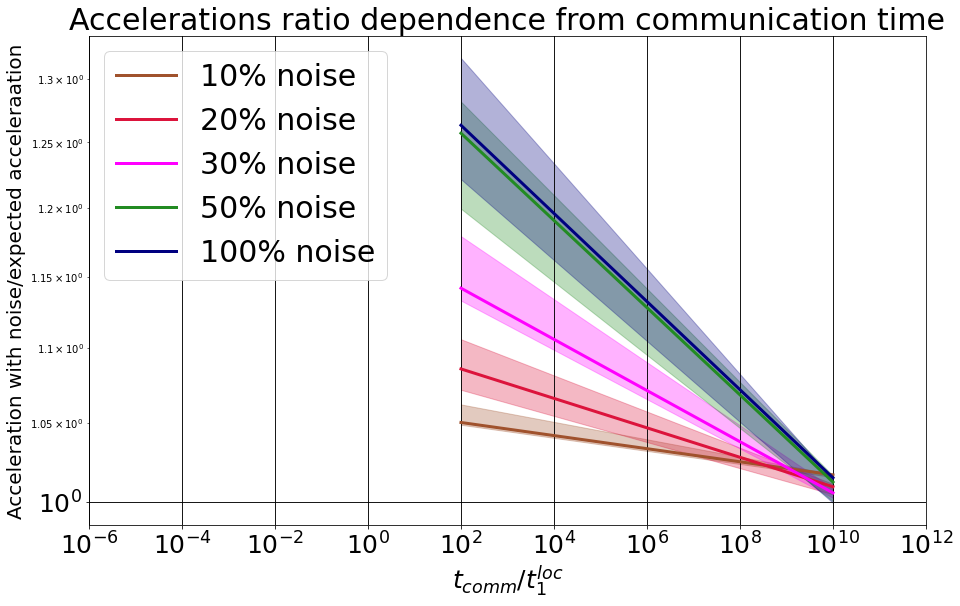
\includegraphics[scale = 0.35]{график_шумы.png}}}
    \caption{Experiments with the noise in the network}
    \label{ris:image2}
\end{figure}

\section{Conclusion}

In this paper, we presented a new data partitioning method for a distributed optimization problem.
Our solution is based on constructing the running time function of Algorithm \ref{alg:1} and finding its minimum. Our method works well in networks with varying communication costs between the server and local devices and different capacities of the devices. The theoretical results have been confirmed experimentally. This shows that our method gives acceleration on this type of problems. In addition, by assuming noise in the networks, we obtain the error of the optimal solution and conduct appropriate experiments.

\printbibliography[heading=bibintoc,title={References}]


\end{document}